\chapter{Related Work}\label{chapter:relatedwork}

\section{Datasets for driver behavior analysis}

As of the time of writing, numerous datasets are available for driver behavior analysis, each with its own specific focus. For instance, \textbf{DR(eye)VE Dataset}\cite{palazzi2018predicting}capturing drivers' gaze patterns in real-world scenarios, includes ego-centric views and car-centric views, which provide data on where drivers look in different driving contexts. \textbf{Naturalistic Driving Study (NDS)}\cite{regan2012naturalistic} contains extensive data collected from naturalistic driving conditions, including in-vehicle driver behavior such as driver movements, eye gaze, and interactions with vehicle controls during different driving scenarios. Detailed information can be found in \ref{chapter:appendix}


In our work, we utilize the \textbf{Drive \& Act} dataset\cite{9009583} as our primary training resource. This dataset includes over twelve hours and 9.6 million frames, capturing individuals engaged in various distractive activities during both manual and automated driving. It is specialized for distinguishing between closely related actions (e.g., opening a bottle vs. closing a bottle) and features a high diversity in action durations and complexities, presenting unique challenges for action recognition models. For instance, brief actions like opening a door from the inside may take less than a second, while prolonged activities such as reading a magazine may last several minutes. This dataset is exceptionally well-suited to our study, as it provides a comprehensive view of driver behavior within the vehicle, with accurately labeled, temporally sequenced annotations for each behavior.


\begin{figure}
    \centering
    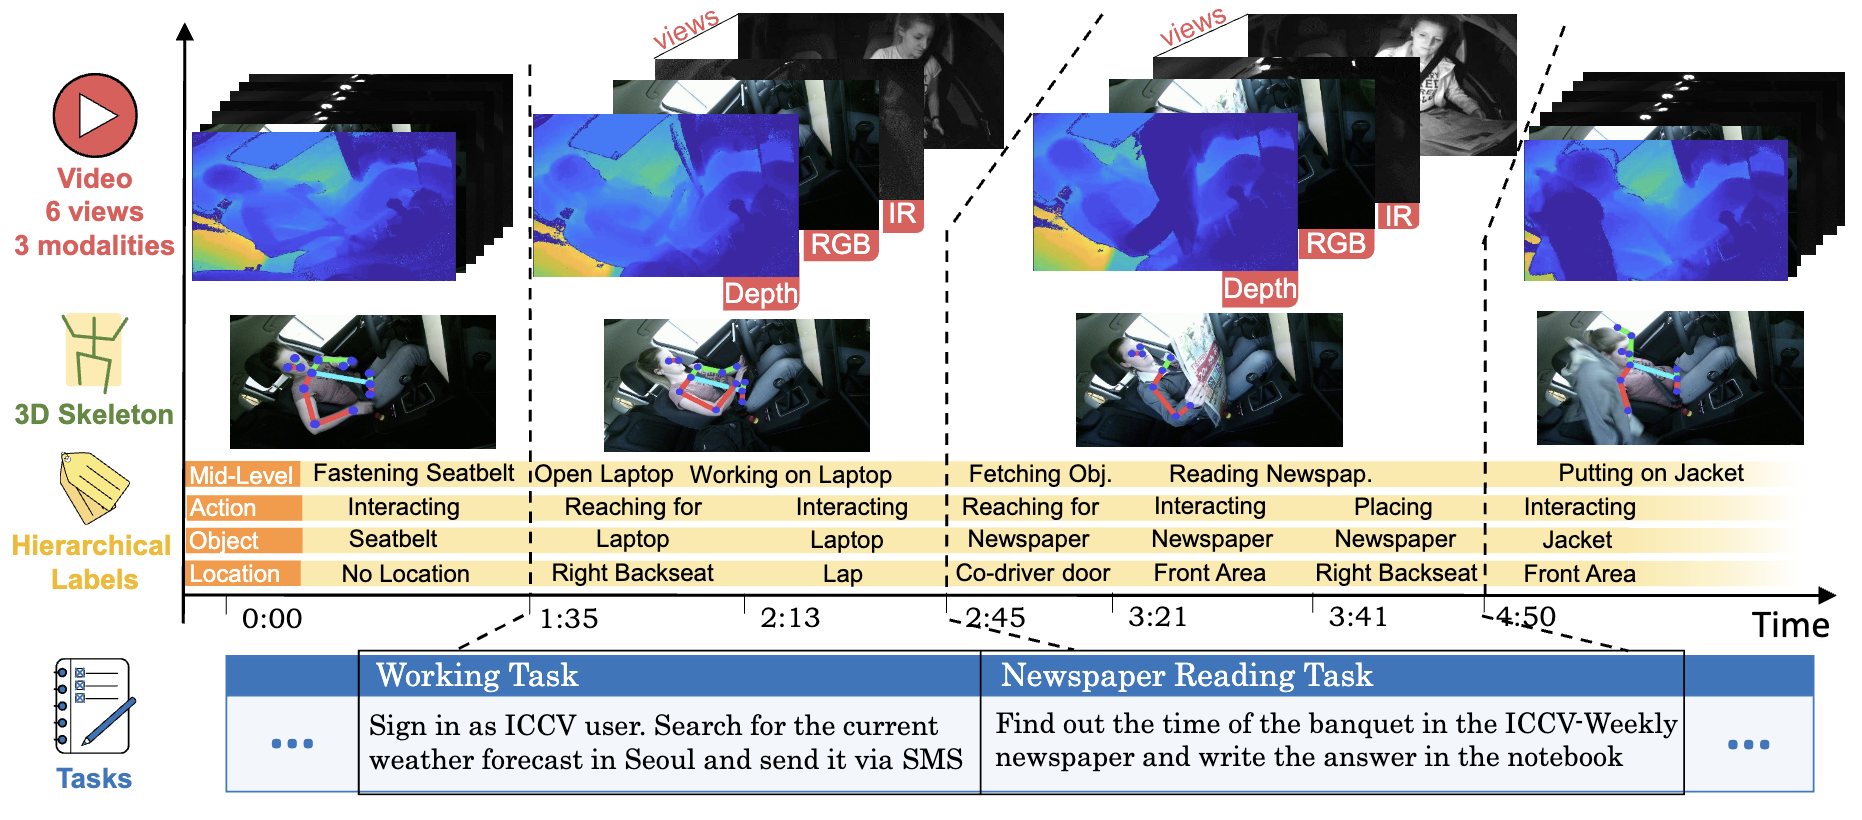
\includegraphics[width=\linewidth]{figures/03_DriveAct.png}
    \caption{Overview of the Drive\&Act dataset for driver behavior recognition. Reproduced from\cite{9009583}}
    \label{fig:DriveAct}
\end{figure}

\section{Dynamic Scene Graph for Video}

As is revealed in chapter\ref{chapter:background}, the most common way to represent the latent information in a video is to use CNNs to directly extract the features of the frames and then use RNNs to model the temporal information. However, this method has its limitations as the excessive high-dimensional abstraction may cause the model to misinterpret human learning intentions; in other words, the black box itself is difficult to interpret. In our work we would like to extract the dynamic scene graph from the video, which is a more intuitive way to represent the video content.

The scene graph is a structured representation of a scene that can clearly express the objects, attributes, and relationships between objects in the scene\cite{9661322}. Accompanied by the development of computer vision technology, simply detecting and recognizing objects in images no longer satisfies the researchers, as they would expect some higher level of understanding and reasoning for image vision tasks. In this way, an intuitive idea comes up about adding up the relationship between the detected objects (See example in figure\ref{fig:SGG}). The earliest research could date back to 2017, when some objects and relations of a given image could be inferred, and a scene graph would be produced as a result\cite{xu2017scene}. Other research like Neural Motifs\cite{zellers2018neural} also shows the possibility of predicting the most frequent relation between object pairs with the given labels and object detections. Later in 2018, videos came into discussion, and both spatial and temporal relations would be concerned in the dynamic graph researchers propose to represent\cite{wang2018videos}. Meanwhile, the accuracy of Scene Graph Detection tasks has significantly improved thanks to the application of unbiased SGG\cite{wang2018videos}, fueled by the \textbf{Detection2} \cite{wu2019detectron2}, a library that contains various state-of-the-art detection and segmentation algorithms. In a nutshell, representing videos as dynamic scene graphs including the detection of objects and the relations in between has been realized in the past years. And our work would utilize such technique and extract our driver-oriented dynamic scene graphs for further learning.

\begin{figure}
    \centering
    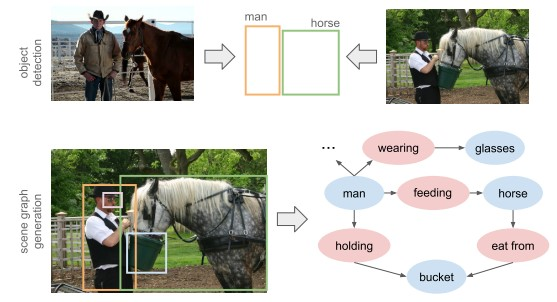
\includegraphics[width=\linewidth]{figures/03_SGG.jpg}
    \caption{Scene Graph Generation by Iterative Message Passing. Reproduced from\cite{tang2020unbiased}}
    \label{fig:SGG}
\end{figure}

\section{Dynamic Link Prediction}


After extracting the dynamic scene graph from video data, the subsequent phase involves learning the interactions between elements within the scene to enable accurate behavior prediction. This objective can be conceptualized as a link prediction task within a dynamic scene graph, making the selection of an appropriate model critical to the success of our approach. Leveraging the review provided in DGB \cite{poursafaei2022towards}, we have identified and evaluated various link prediction models along with effective evaluation strategies. Below, we introduce each model and provide a theoretical explanation for our choice.

\subsubsection{ JOINT DYNAMIC USER-ITEMEMBEDDING MODEL(JODIE)}
Based on the user-item interaction data, JODIE\cite{kumar2019predicting} works as a coupled Recurrent Neural Networks(RNN). The update operator alternatively updates the embedding space of suer and an item at each interaction. And the projection operator learns to estimate the embedding of the user at any time in the future, thereby enabling the prediction of forthcoming interactions. The design and functionality of JODIE align well with our objectives, making it a strong candidate for our work.

\subsubsection{Representation Learning over Dynamic Graphs(DyRep)}
DyRep\cite{trivedi2018representation} is an inductive deep representation learning framework that learns a set of functions to efficiently produce low-dimensional node embeddings that evolves over time. The model captures all the new edges appears during the time sequence and updates the embeddings of the nodes accordingly in a custom RNN model. The final output provides a solution to the problems of dynamic link prediction and event time prediction. TGN achieves superior performance over prior models and offers computational efficiency, making it a potential fit for our data, although some constraints exist.


\subsubsection{Temporal Graph Network(TGN)}
\textbf{TGN}\cite{rossi2006temporal} is a generic, efficient framework for deep learning on dynamic graphs represented as sequences of timed events. To train the Memory-related modules, the message matrix would begin with a raw message store and is updated based on interactions which have been processed by the model in the past, which would also propagate to the node embedding as well as the loss function. TGNs significantly outperform previous approaches while being more computationally efficient, Which offer the possibility for our data.

\subsubsection{Causal Anonymous Walks Network (CAW-N)}
Based on temporal random walks, \textbf{CAW-N} adopt a novel anonymization strategy that replaces node identities with the hitting counts of the nodes based on a set of sampled walks to keep the method inductive, and simultaneously establish the correlation between motifs. It is specialized in work as automatic retrieval of temporal network motifs to represent network dynamics. Since our dataset has only little similarity with random walking, we didn't take this into consideration at last.


After evaluating each of these models, we selected \textbf{JODIE} as the final model for our work. Theoretically, this choice is justified by the structural similarity of our dataset, which features participant-object interactions akin to user-item data. Although \textbf{TGN } also offers a sophisticated architecture, its need for extensive training data rendered it impractical for our dataset's constraints.